\documentclass[10pt]{standalone}
\usepackage{commands}
\begin{document}
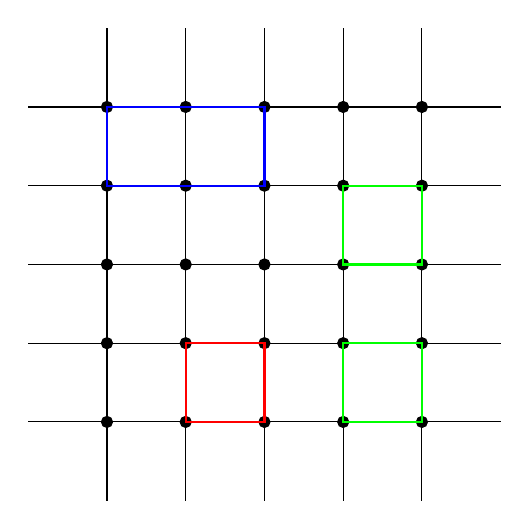
\begin{tikzpicture}
    \foreach \j in {1,...,5} {
            \draw[] (-1, \j) -- (5, \j);
    };
    \foreach \i in {0,...,4} {
        \foreach \j in {1,...,5} {
            \filldraw (\i, \j) circle (2pt);
        }
        \draw[] (\i, 0) -- (\i, 6);
    };
    \draw[red, thick] (1, 1) -- (2, 1) -- (2, 2) -- (1, 2) -- cycle;
    \draw[blue, thick] (0, 4) -- (2, 4) -- (2, 5) -- (0, 5) -- cycle;
    \draw[green, thick] (3, 1) -- (4, 1) -- (4, 2) -- (3, 2) -- cycle;
    \draw[green, thick] (3, 3) -- (4, 3) -- (4, 4) -- (3, 4) -- cycle;
\end{tikzpicture}
\end{document}